\section{Model Verification}
\label{section_model_varification}
In this section, START mobility model is validated on the aspects of node distribution and contact characteristics. All movement models are implemented on Opportunistic Networking Environment (ONE)\cite{KeranenOtt-155}.

In order to  validate that the behavior difference for each status will affect the accuracy of mobility models, a simplified model, S-START, is developed based on START by modifying the speed generator according the speed distribution $g_{status=0,1}(x)$ and $f_{status=0,1}(x)$. Because status difference is neglected, there is no need to discuss the status duration.

Shortest Path movement model based on the map in Beijing is an other comparison, which is implemented by ONE.  It moves will find shortest path from source to destination by Dijkstra algorithm.
 The RWP model is another comparison, because it is proved to be an efficient model modeling the nodal movement in VANETs. It's simple and effective, but takes no consideration of the node statuses and geographical distribution.

The START, S-START, Shortest Path and RWP mobility model are compared with the real trace of Beijing, China.
In simulations, Node number is set as 4000 and scenario in area $24445*23785 m^2$ (a sub-map of the whole area), including fourth ring roads in Beijing. The simulation time is three hours and the warm up time for reports is one hour, so that the nodal movement and position will not be affected by its initial position. The communication range is $200m$.

\subsection{Traces and distribution of nodes}

Trace samples and their snapshots are demonstrated in this section, shown as fig. \ref{figure_tracesample} and fig.\ref{figure_tracesnapshoots}.

From fig.\ref{figure_tracesnapshoots}, Real trace and Shortest Path movement model exhibit the road structure, while START and S-START display the geographic feathers defined in section \ref{section_design}. However, the node distribution of RWP is much uniform.



\begin{figure*}[!h]
\centering
\subfigure[Real Trace]{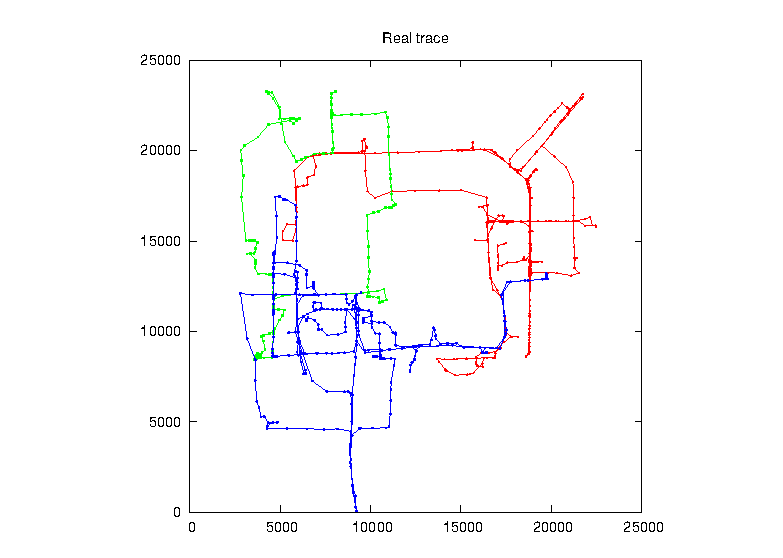
\includegraphics[width=0.4\textwidth]{figures_201103/Evaluation/trace_real.eps}}
\subfigure[START]{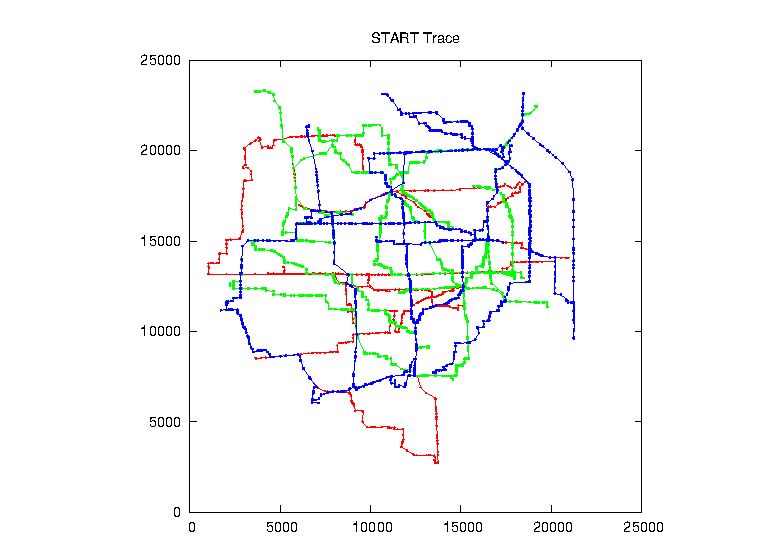
\includegraphics[width=0.4\textwidth]{figures_201103/Evaluation/trace_start.eps}}
\subfigure[RWP]{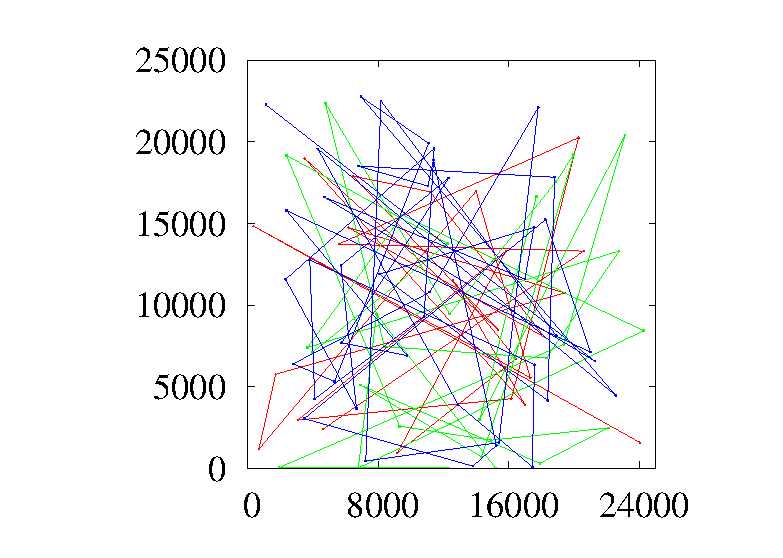
\includegraphics[width=0.4\textwidth]{figures_201103/Evaluation/trace_rwp.eps}}
\subfigure[SP]{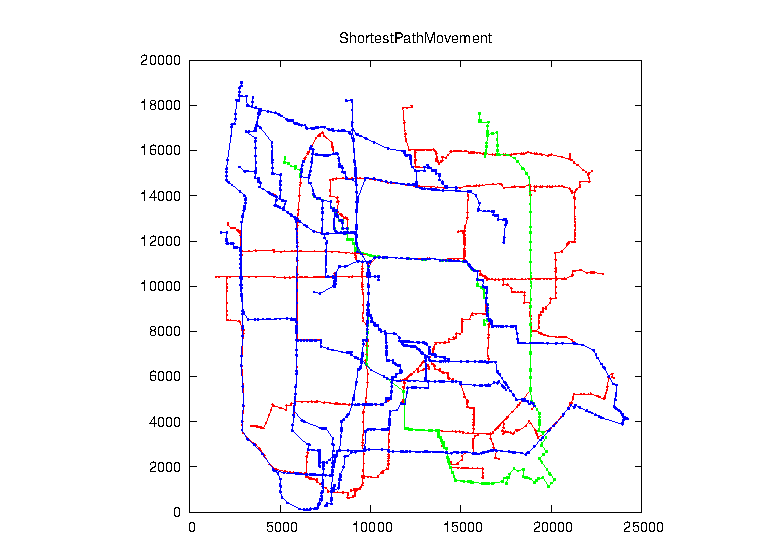
\includegraphics[width=0.4\textwidth]{figures_201103/Evaluation/trace_sp.eps}}
\caption{Trace samples}\label{figure_tracesample}
\end{figure*}


\begin{figure*}[htbp]
\centering
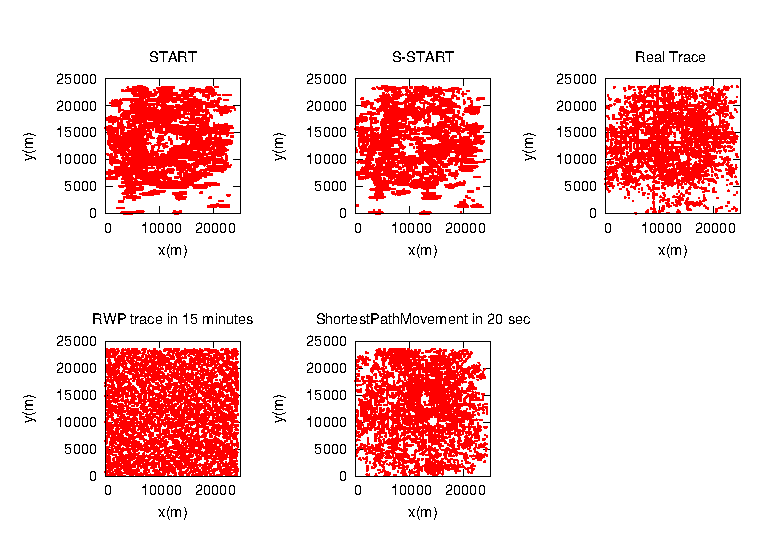
\includegraphics[width=0.8\textwidth]{figures_201103/Evaluation/ev_tracesnapshoots.eps}\\
\caption{Nodes distribution snapshoots}\label{figure_tracesnapshoots}
\end{figure*}

By dividing areas into $10*10$ grids, (length of each cell is about 2400 meters), the node density distributions are investigated, shown in fig.\ref{figure_node_distribution}. An interpolation process is conducted on RWP traces, because it will not generate a position data until it changes its direction. Under this condition, middle point in the straight line created by two original points of continues time stamp is inserted for every 5 seconds. In each cell of grids in 20 seconds, the distinct nodes occurring are counted, that is, if a node prints its location in a cell twice, it will not add up to the node density in this square. Consequently, the interpolation process on RWP trace will not influence the results. Moreover, the upper limit of speed is 33.3 m/s, so that for every node, it can occur in no more than 3 cells in 20 seconds.  In table. \ref{figure_avg_var_node_density}, the average of node densities for models and real traces are close. Whereas, the variances change a lot from 4848 of RWP to 107423.3 of START. The variance of Real trace is large, because nodes in reality during a short time is not evenly distributed. Although, Shortest Path movement model takes the geographic characteristics into consideration, the difference from different road segments is disregarded.

\begin{table}
\centering
\caption{Average and variance of node density}\label{figure_avg_var_node_density}
\begin{tabular}{r|c|c}
  \hline
  % after \\: \hline or \cline{col1-col2} \cline{col3-col4} ...
 type & average & variance\\
  \hline
  Real Trace & 41.39175 & 107401.1 \\
  START & 44.28421 & 107423.3 \\
  S-START & 45.3 & 86084.9\\
  ShortestPath & 43.41414 & 52820\\
  RWP & 43.2 & 4848 \\
  \hline
\end{tabular}
\end{table}

\begin{figure*}[htbp]
\centering
\subfigure[RWP]{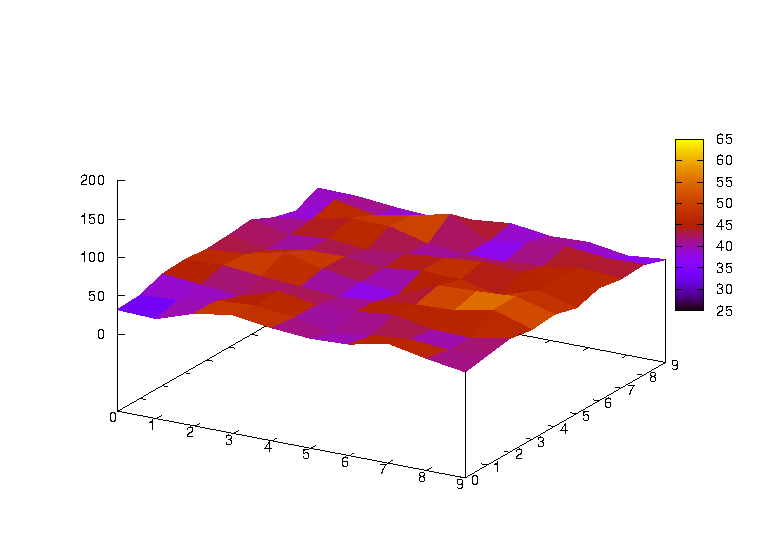
\includegraphics[width=0.3\textwidth]{figures_201103/Evaluation/ev_nodedis_rwp.eps}}
\subfigure[ShortestPathMovement]{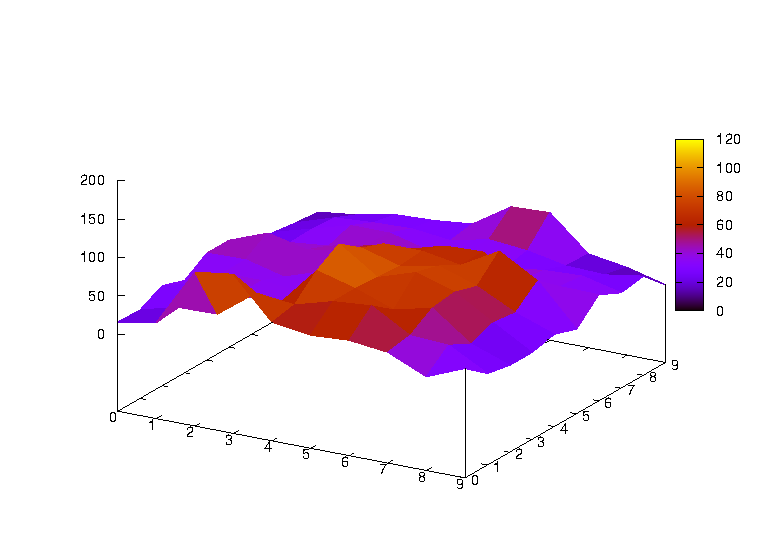
\includegraphics[width=0.3\textwidth]{figures_201103/Evaluation/ev_nodedis_sp.eps}}
\subfigure[S-START]{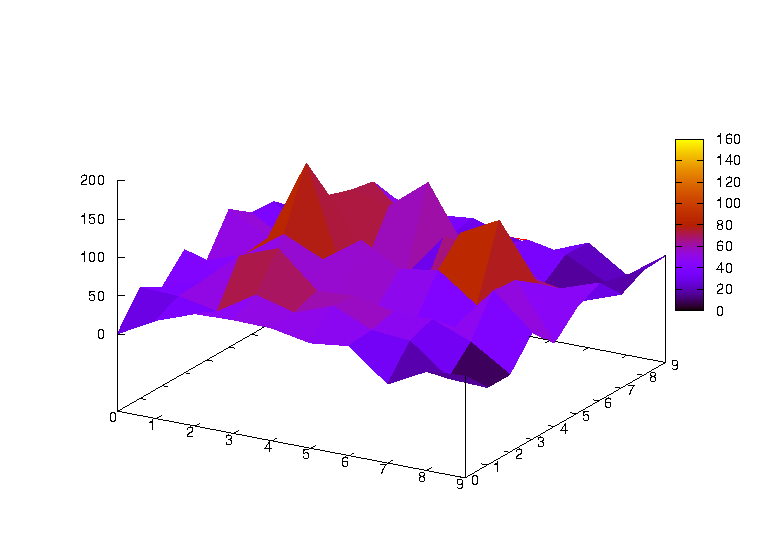
\includegraphics[width=0.3\textwidth]{figures_201103/Evaluation/ev_nodedis_s_start.eps}}
\subfigure[START]{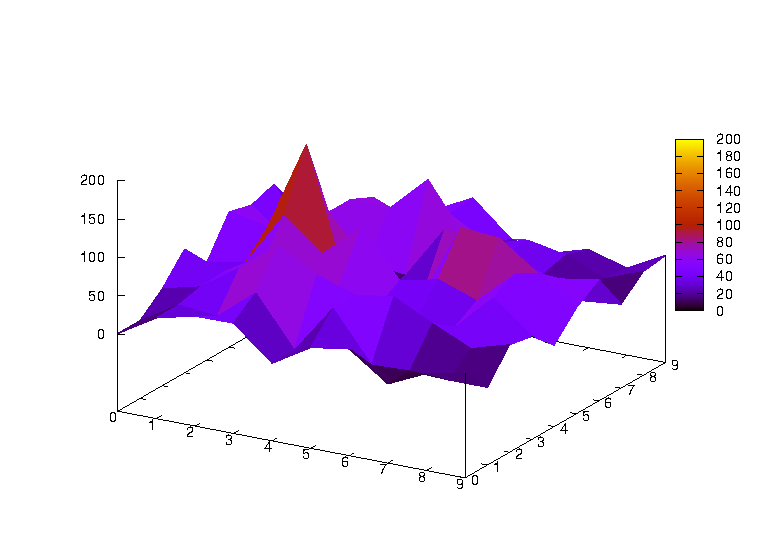
\includegraphics[width=0.3\textwidth]{figures_201103/Evaluation/ev_nodedis_start.eps}}
\subfigure[Trace]{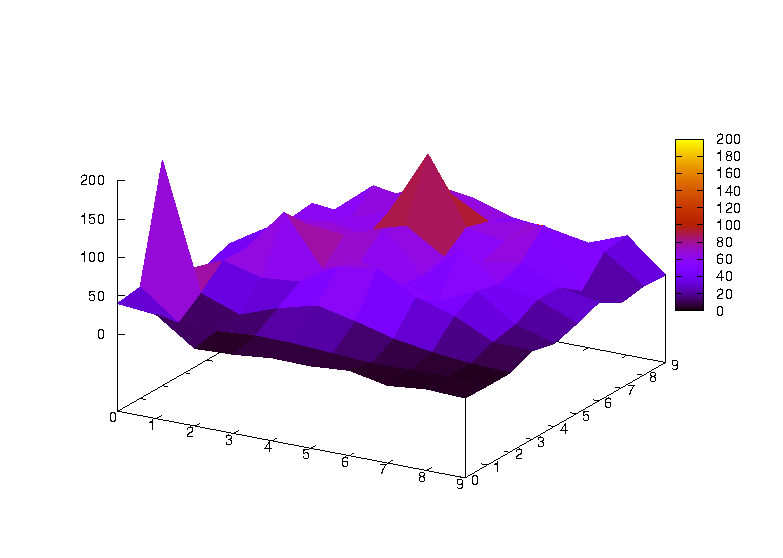
\includegraphics[width=0.3\textwidth]{figures_201103/Evaluation/ev_nodedis_trace.eps}}
\caption{Node density in 20 seconds}\label{figure_node_distribution}
\end{figure*}


\subsection{Contacts characteristics}

The contacts (connections) and inter contact time (ICT) \cite{vHuWang-23} are evaluated as the indicator to compare the similarity.
During simulation time, there are 1744093 contacts in real trace scenario, 1808621 contacts of START, 1271044 contacts of S-START model and 1007756 contacts of RWP model.

\begin{figure*}[htbp]
\centering
\subfigure[Contact times vs. frequency]{
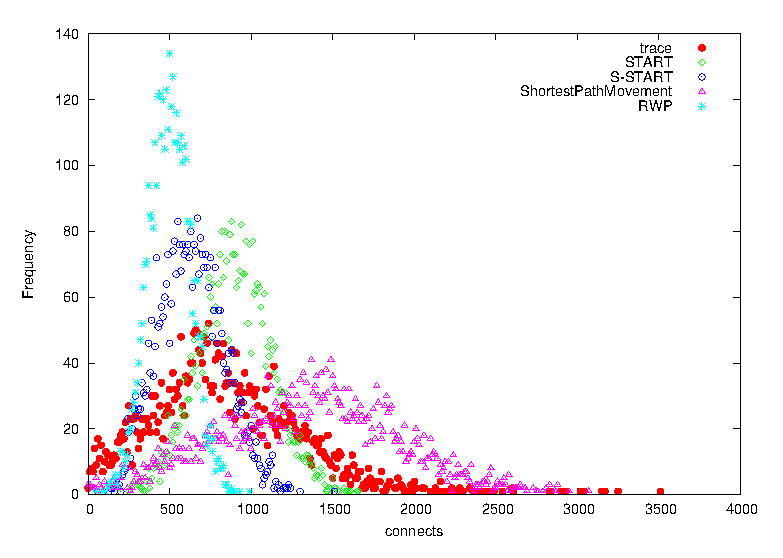
\includegraphics[width=0.3\textwidth]{figures_201103/Evaluation/ev_connections.eps}
}
\subfigure[neighbors vs. frequency]{
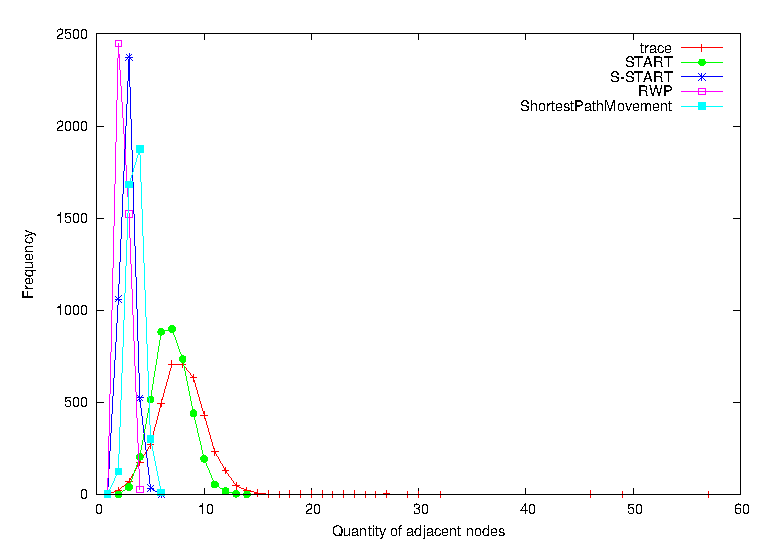
\includegraphics[width=0.3\textwidth]{figures_201103/Evaluation/ev_neigbors.eps}
}
\subfigure[Cumulative ICT distribution]{
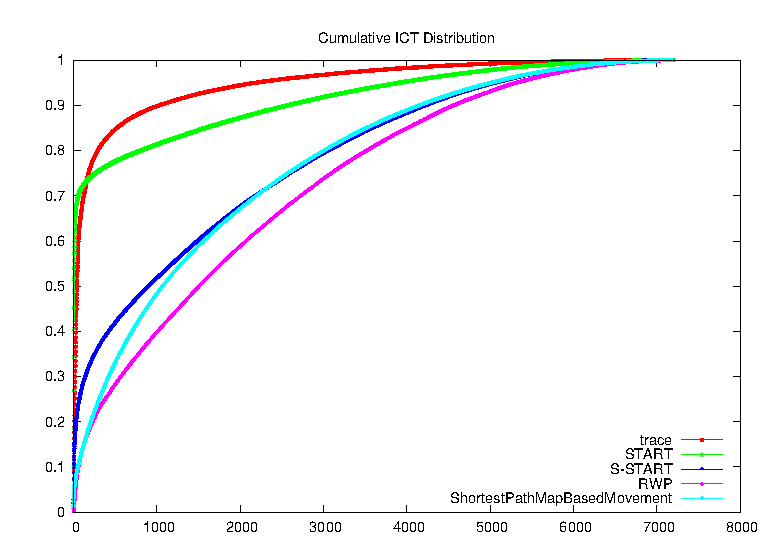
\includegraphics[width=0.3\textwidth]{figures_201103/Evaluation/ev_ict.eps}
}

\caption{Contact times distribution and Cumulative ICT distribution}\label{figure_contacts}
\end{figure*}

The contact frequency proportion distribution is shown as in fig.\ref{figure_contacts}. In fig. \ref{figure_contacts}. (a), the contact times of a node vs. the node frequency is illustrated. For an instance, a point (500,44) of the real trace presents that there are 44 nodes contacts 100 times with other nodes. For real trace $(740,52)$, most nodes (740nodes) contact 52 times.  The peak occurs in $(83, 880)$ for START, $()$ for S-START, $(1370,41)$ for ShortestPath movement model and $(134, 500)$ for RWP.

Fig. \ref{figure_contacts}. (b) demonstrate the neighbors of nodes. If a $node_i$ contacts with a $node_j$, $node_i$ and $node_j$ are neighbors. Based on the trace data set, 709 nodes are with about 8 neighbors. START shows most similarity with real trace with a peak of  $(7,709)$.  For ShortestPath movement model, 1875 nodes have 4 neighbors and For RWP, 2448 nodes contact with other 2 nodes. If the node distribution is even, the peak occurs early, because most nodes are similar. On the contrary, unevenly movement of nodes will cause that some nodes contact with many other nodes but some nodes only contact with a few neighbors.

ICT is also widely used in VANETs to forecast contacts and assist routing decision. The cumulative ICT distributions are further explored, shown in fig.\ref{figure_contacts}(c).
From 0 to 120 sec, the cumulative probability of ICT increases rapidly for the real trace and START. For the other two models, the growth rate varies slightly. In reality, taxies can contact twice in a short time, because the geographical distance are quite close after the first contact. In that case, the ICT tender to be short, causing the cumulative probability of ICT increases rapidly.

To conclude, by comparing the node distribution and contact characteristics, the START mobility model performs good similarity with the real data set. Although the S-START model only ignores the statuses by modifying the parameters of the speed generator, the statistical results show obvious dissimilitude from S-START and the reality. By comparing with Shortest Path movement model, the $assumption 2$ that the unevenly distribution of taxies influences the accuracy of models can be supported in certain degree.
